\documentclass[a4paper,11pt]{article}
\usepackage[left=2.5cm, right=2.5cm, top=2cm, bottom=2.5cm]{geometry}
\usepackage{graphicx}
\usepackage{amssymb}
\usepackage{amsmath}

\begin{document}
	\title{\LARGE{\textbf{ECEN 203 Lab 3 Report}\\Hi-Fi Audio Circuit Design}}
	\author{Niels Clayton : 300437590\\ \textbf{Lab Partner: }Tom Simpson}
	\date{}
	\maketitle

	\begin{flushleft}
	\section*{Part 1: Pre-Amp Subwoofer Filter}
		\begin{enumerate}
		
		\item %first task of part 1
			\textbf{Design a low-pass $RC$ filter with a cut off frequency of $200Hz$}
		
			$\omega = 2 \pi f \quad
			f = 200Hz \quad 
			\therefore \quad \omega=400\pi$
		
			$\tau = RC, \quad 
			\omega = \dfrac{1}{\tau}\quad
			\therefore \quad \omega = \dfrac{1}{RC}$ 
			
			Using this formula we are able to choose a capacitor size and then calculate the size of the 			required resistor using $R = \dfrac{1}{\omega C}$.\\ 
			Using the calculated $\omega=400\pi$, and a capacitor of $1\mu F$, we find that the required 			resistor should be $796 \Omega$.
			
			\begin{figure}[ht]
				\centering
				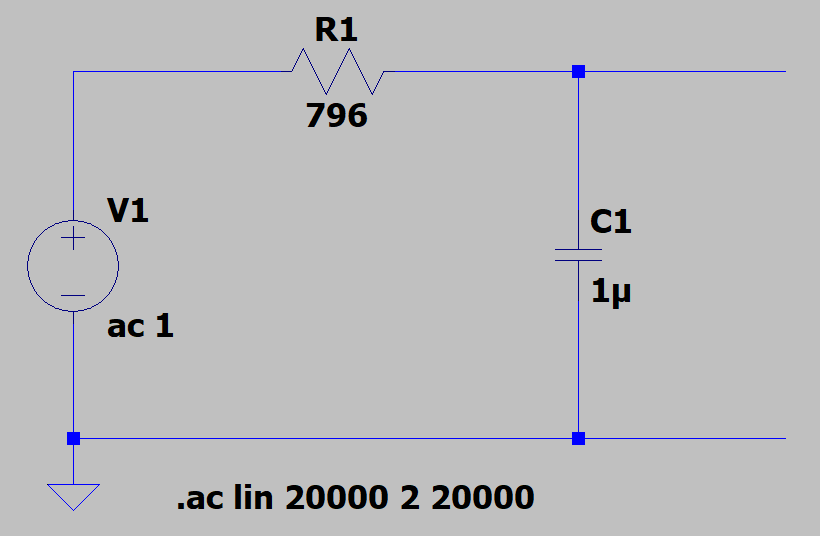
\includegraphics[width=0.8\linewidth]{RC_Filter}
				\caption{RC Low-Pass Filter}
			\end{figure}
		
		\newpage
		\item %task 2, part 1
			\textbf{Plot the transfer function of the filter with no load connected.}
			
			\begin{figure}[ht]
				\centering
				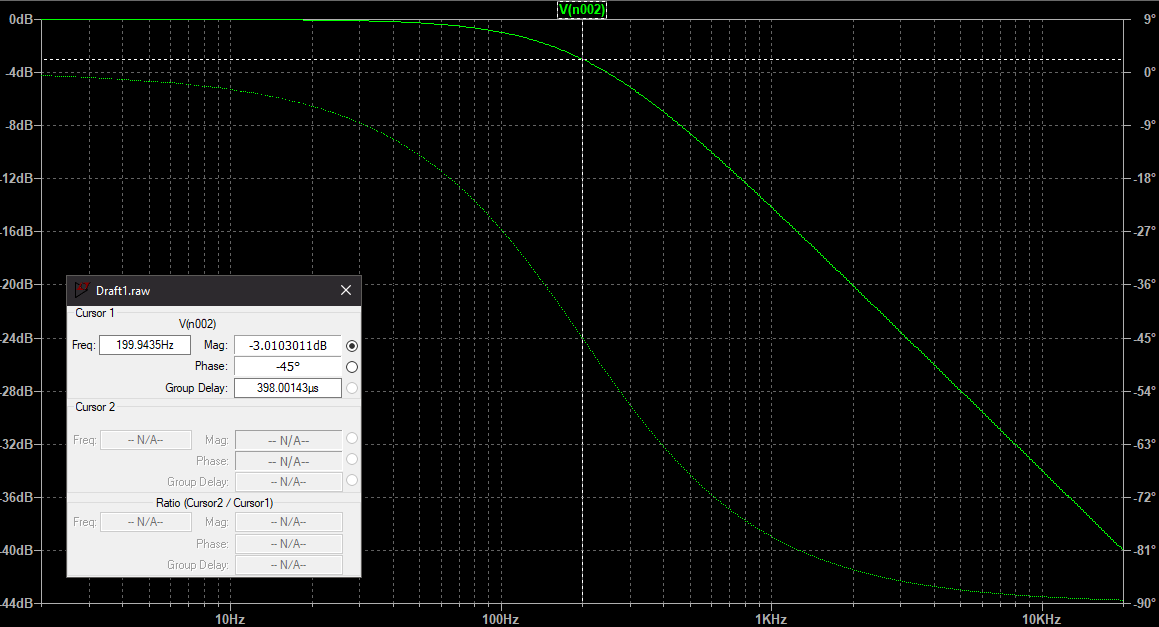
\includegraphics[width=\linewidth]{RC_transfer_function}
				\caption{RC Low-Pass Transfer Function (No Load)}
			\end{figure}
			The transfer function of this filter is $ \dfrac{\dfrac{1}{j\omega RC}}{1+\dfrac{1}{j\omega 				RC}}$ which can be simplified down to $ \dfrac{-j}{\omega\tau -j}$\\
			This transfer function $H(\omega) = \dfrac{-j}{\omega\tau -j}$ can now be used to find the 					gain of the circuit at given frequencies using the magnitude of the transfer function: $Gain 			= 10\log|H(\omega)|$\\
			\begin{itemize}
				\item
				$10\log|H(40\pi)| = -0.04 dB$
				\item
				$10\log|H(40\pi)| = -3.01 dB$
				\item
				$10\log|H(4000\pi)| = -20.04 dB$
			\end{itemize}
			
		\newpage
		\item %task 3, part 1
			\textbf{Repeat the AC analysis and calculate the cut off frequency, but now with a $10k						\Omega$ resistor across $V_{o}$.} \\
			\begin{figure}[ht]
				\centering
				\includegraphics[width=\linewidth]{Loaded_RC_filter}
				\caption{Loaded RC Low-Pass Transfer Function}
			\end{figure}
			To calculate the new $f_{c}$ we can use the $f_{c}=\dfrac{(R1+R2/C R1 R2)}{2\pi}$, 							calculating the new $f_{c}$ to be $215.86Hz$ which is corroborated by the transfer function 				in figure 3. This is known as a terminated RC filter, with the load acting to lower the gain 			of the filter, and shift the cut-off frequency to a higher frequency.
		
		\item %task 4, part 1
			\textbf{Insert a voltage follower between the filter and the $10k\Omega$ resistor:}
			\begin{figure}[ht]
				\centering
				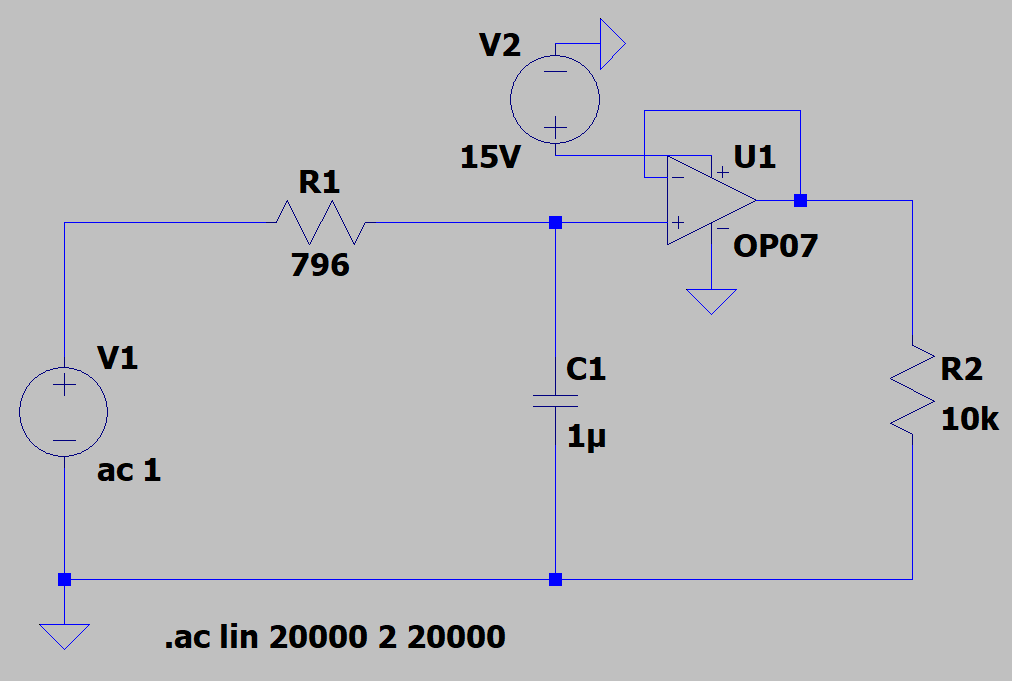
\includegraphics[width=0.8\linewidth]{OP_AMP_FILTER}
				\caption{Voltage Follower}
			\end{figure}
		\newpage
			\begin{figure}[ht]
				\centering
				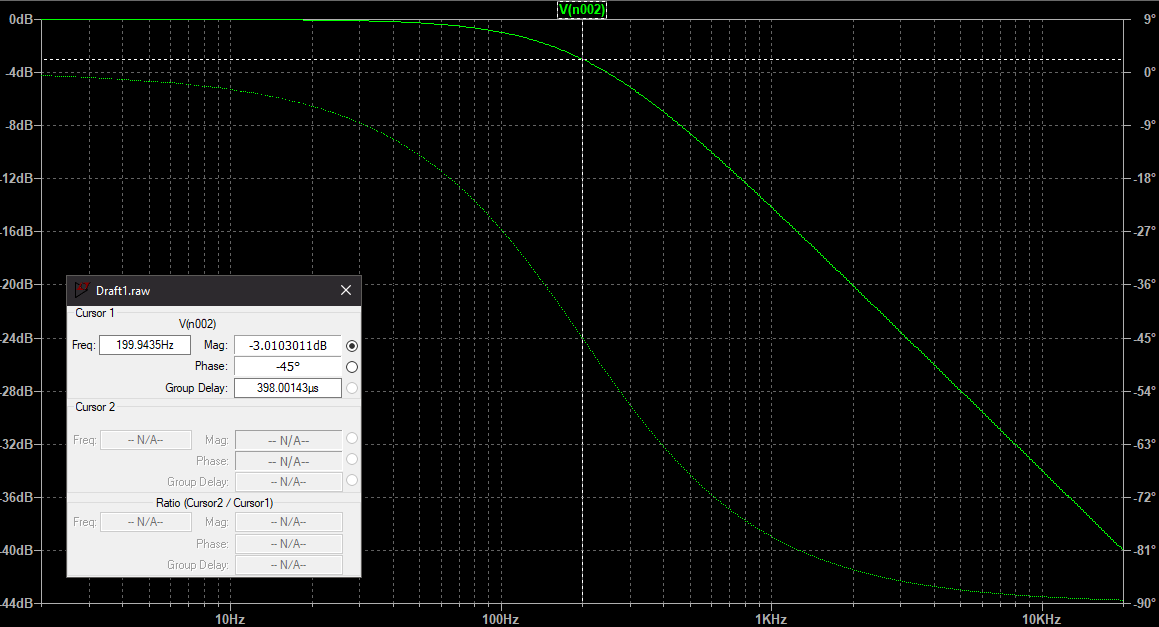
\includegraphics[width=0.8\linewidth]{RC_transfer_function}
				\caption{Voltage Follower Transfer Function}
			\end{figure}
			It is observed that the gain of this filter is the same as the previous low-pass RC filter 					with no load attached. This is due to the voltage divider actually just being an OP-Amp with 			a gain of 1. This means that the voltage being presented on the non-inverting terminal will 				be the output voltage of the OP-Amp, but powered from a seperate power supply, meaning that 				is it isolated from the rest of the filter.
		\end{enumerate}
		\newpage
	\enlargethispage{\baselineskip}
	\section*{Part 2: Audio Effects Unit}
		\begin{enumerate}
		\item %task 2 of part 1
			\textbf{Build an Integrating Circuit Using OP-Amp's and capacitors}
			\begin{figure}[ht]
				\centering
				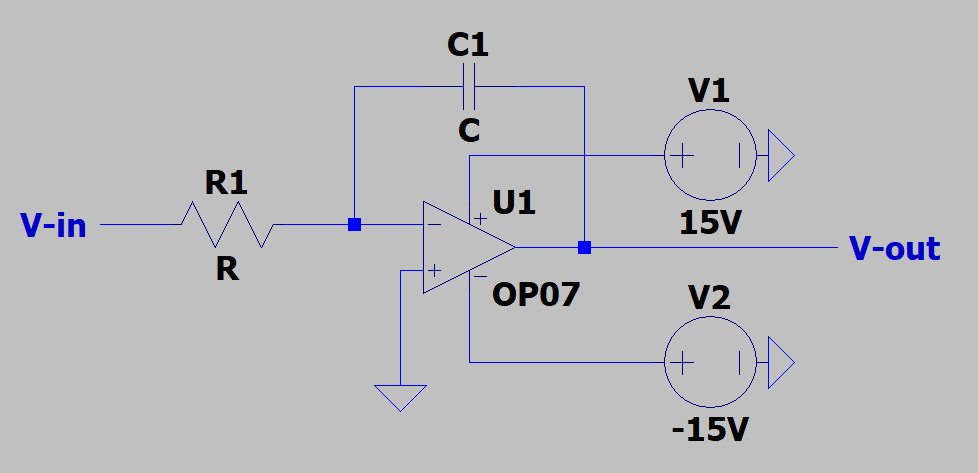
\includegraphics[width=0.6\linewidth]{integrating}
				\caption{Integrating circuit design}
				\includegraphics[width=0.6\linewidth]{integrator}
				\caption{Integrating circuit on bread board}
				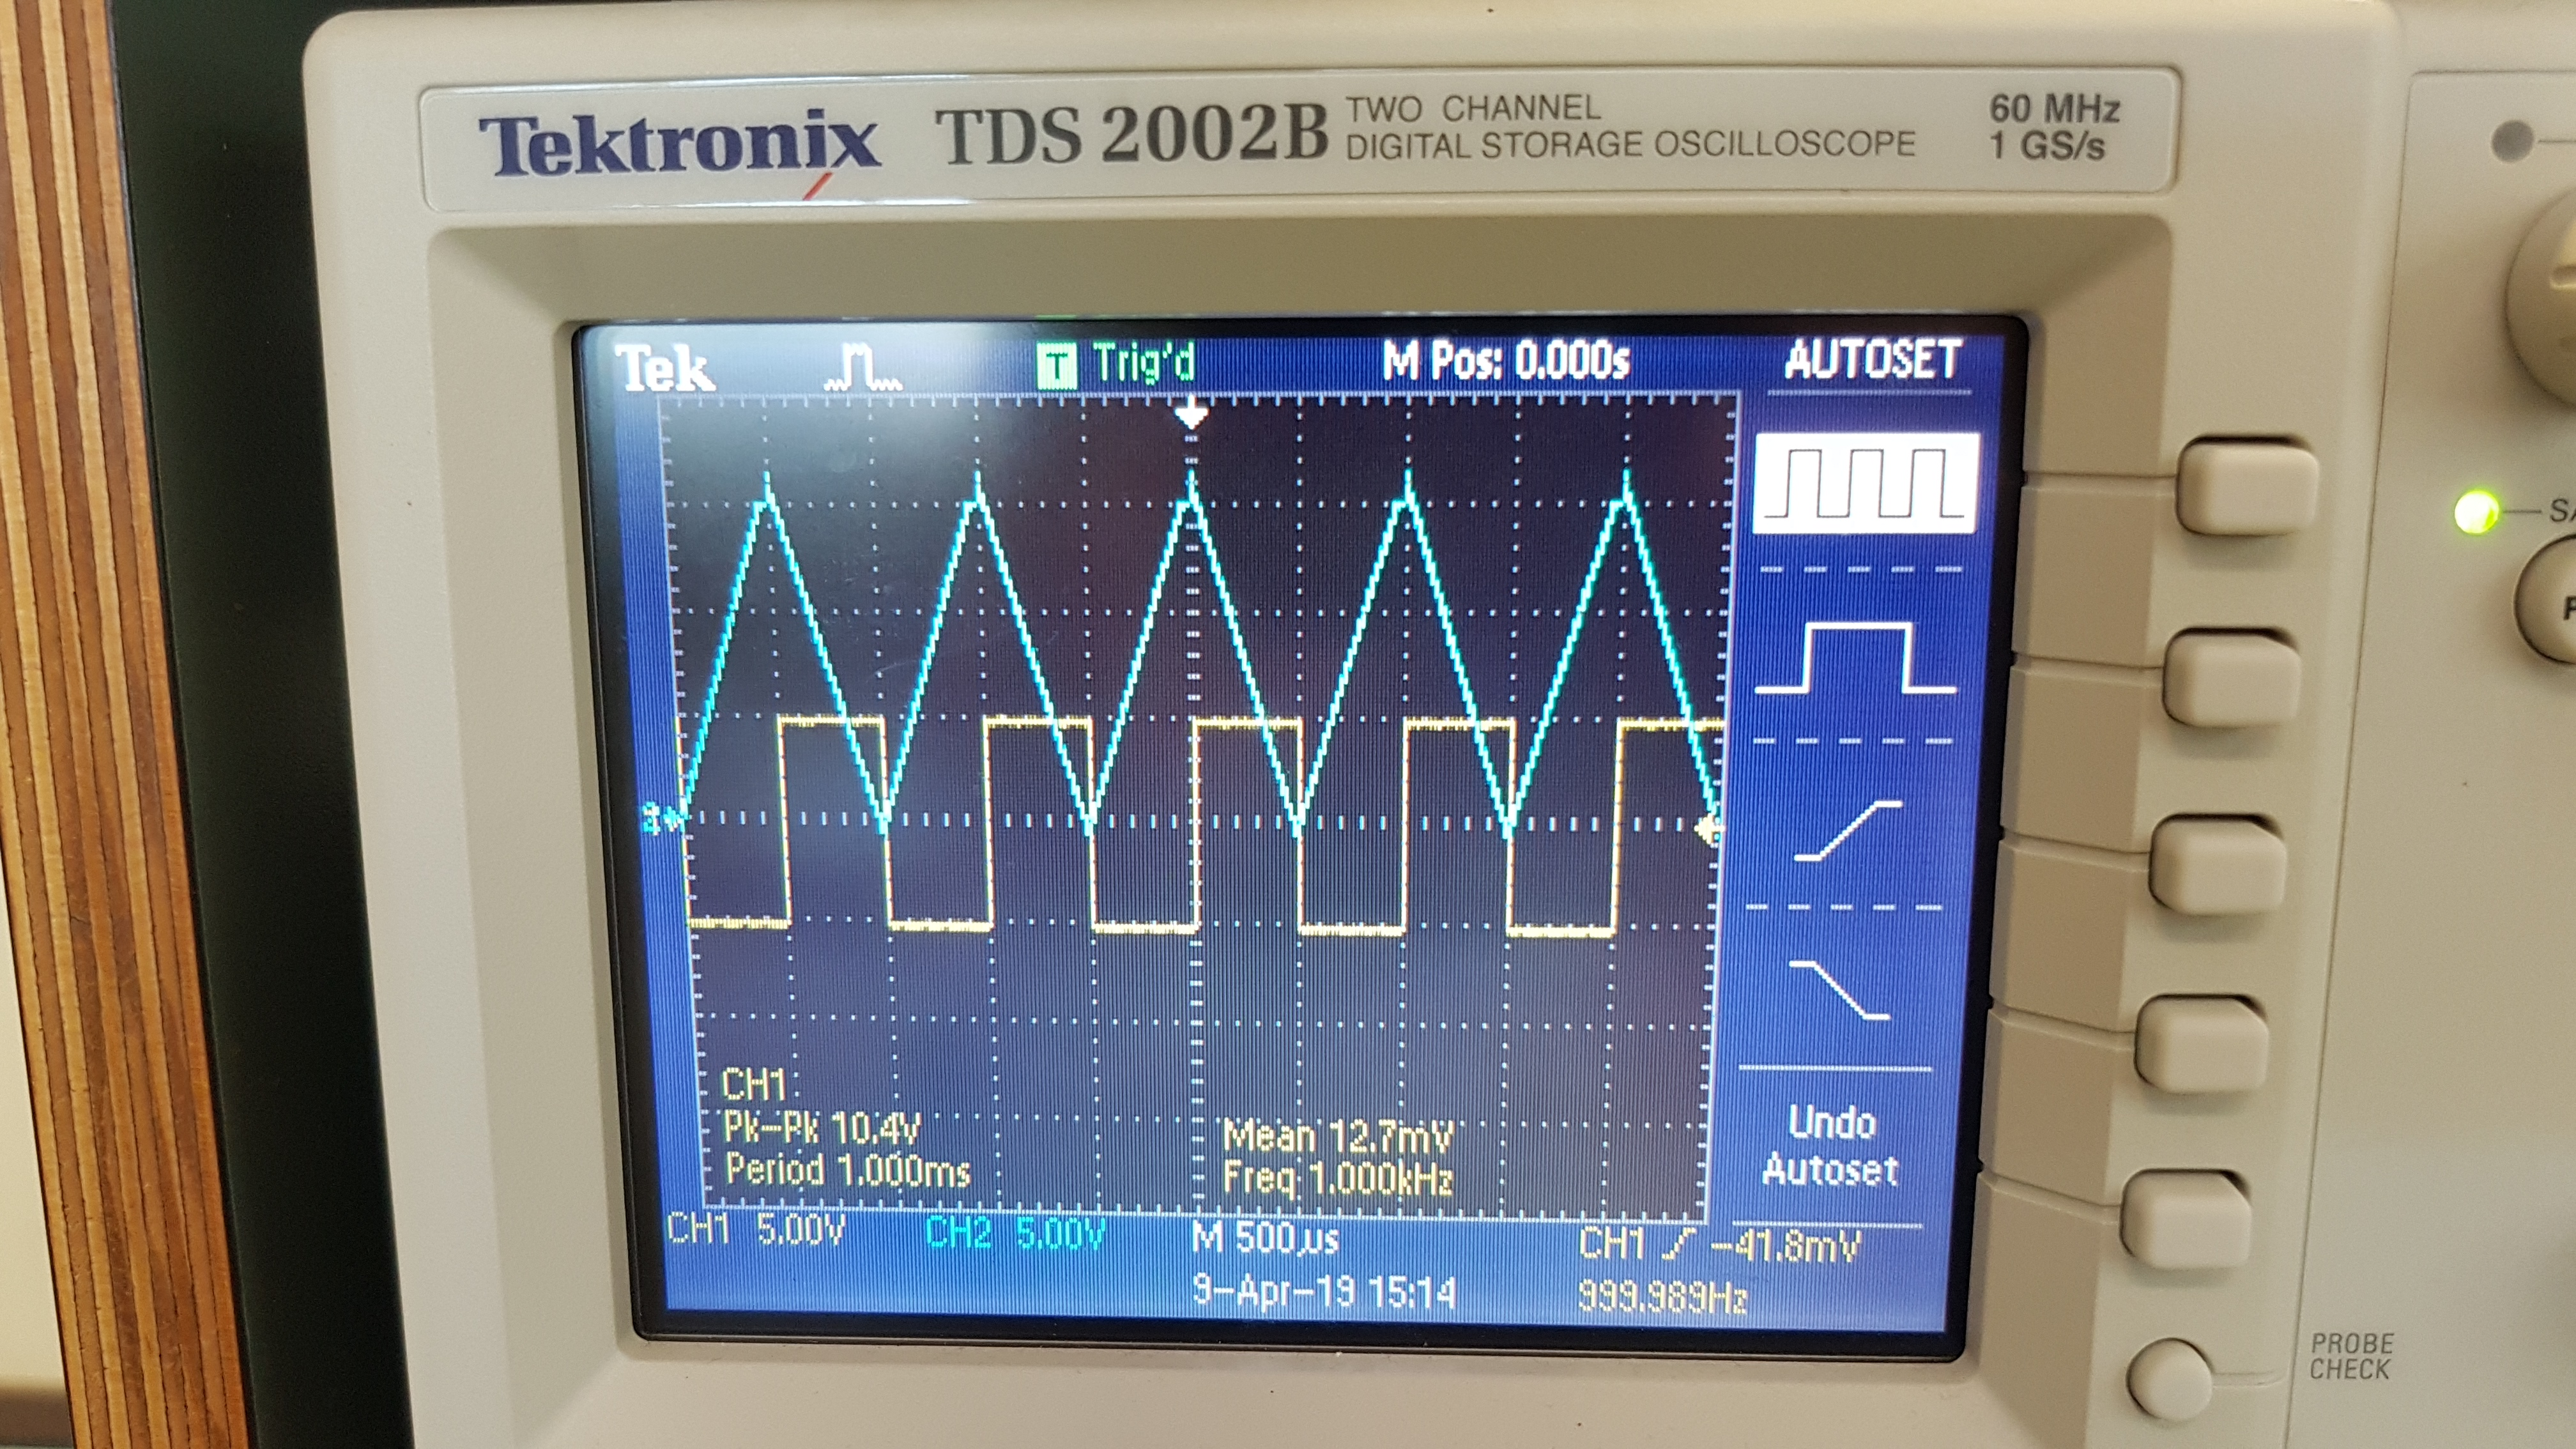
\includegraphics[width=0.6\linewidth]{scope_readout}
				\caption{oscilloscope readings of the output of the OP-Amp}
			\end{figure}
			the behaviour of the integrating circuit can be explained when thinking about the charging 					and discharging or a capacitor. As a voltage is applied at $V_{in}$ this voltage is then 					applied on the plate of the capacitor. Because of this the OP-Amp immediately supplies an 					equal voltage to the opposite side of the capacitor in order to cancel this out. It is 						because of this, that as the capacitor charges you get a linear increase in the output 						voltage $V_{out}$. It is  also observed that there is an overall DC voltage bias to the 					output of the OP-Amp. This is due to imperfections in the chip or due to a bias in the 						supply voltage, and leads to the capacitor never fully discharging. The affect of this as 					seen in figure 8 is that the output is shifted up to either of the  input rails of the OP-					Amp.
		\newpage
		\item
			\textbf{DC Biases and Output Wind-up}\\
			One way to avoid the aforementioned DC voltage bias in the output is to place a 							'dissipating' resistor in parallel with the capacitor. This will ensure that the capacitor 					will always fully discharge and help avoid a DC bias or wind-up.\\
			\begin{figure}[ht]
				\centering
				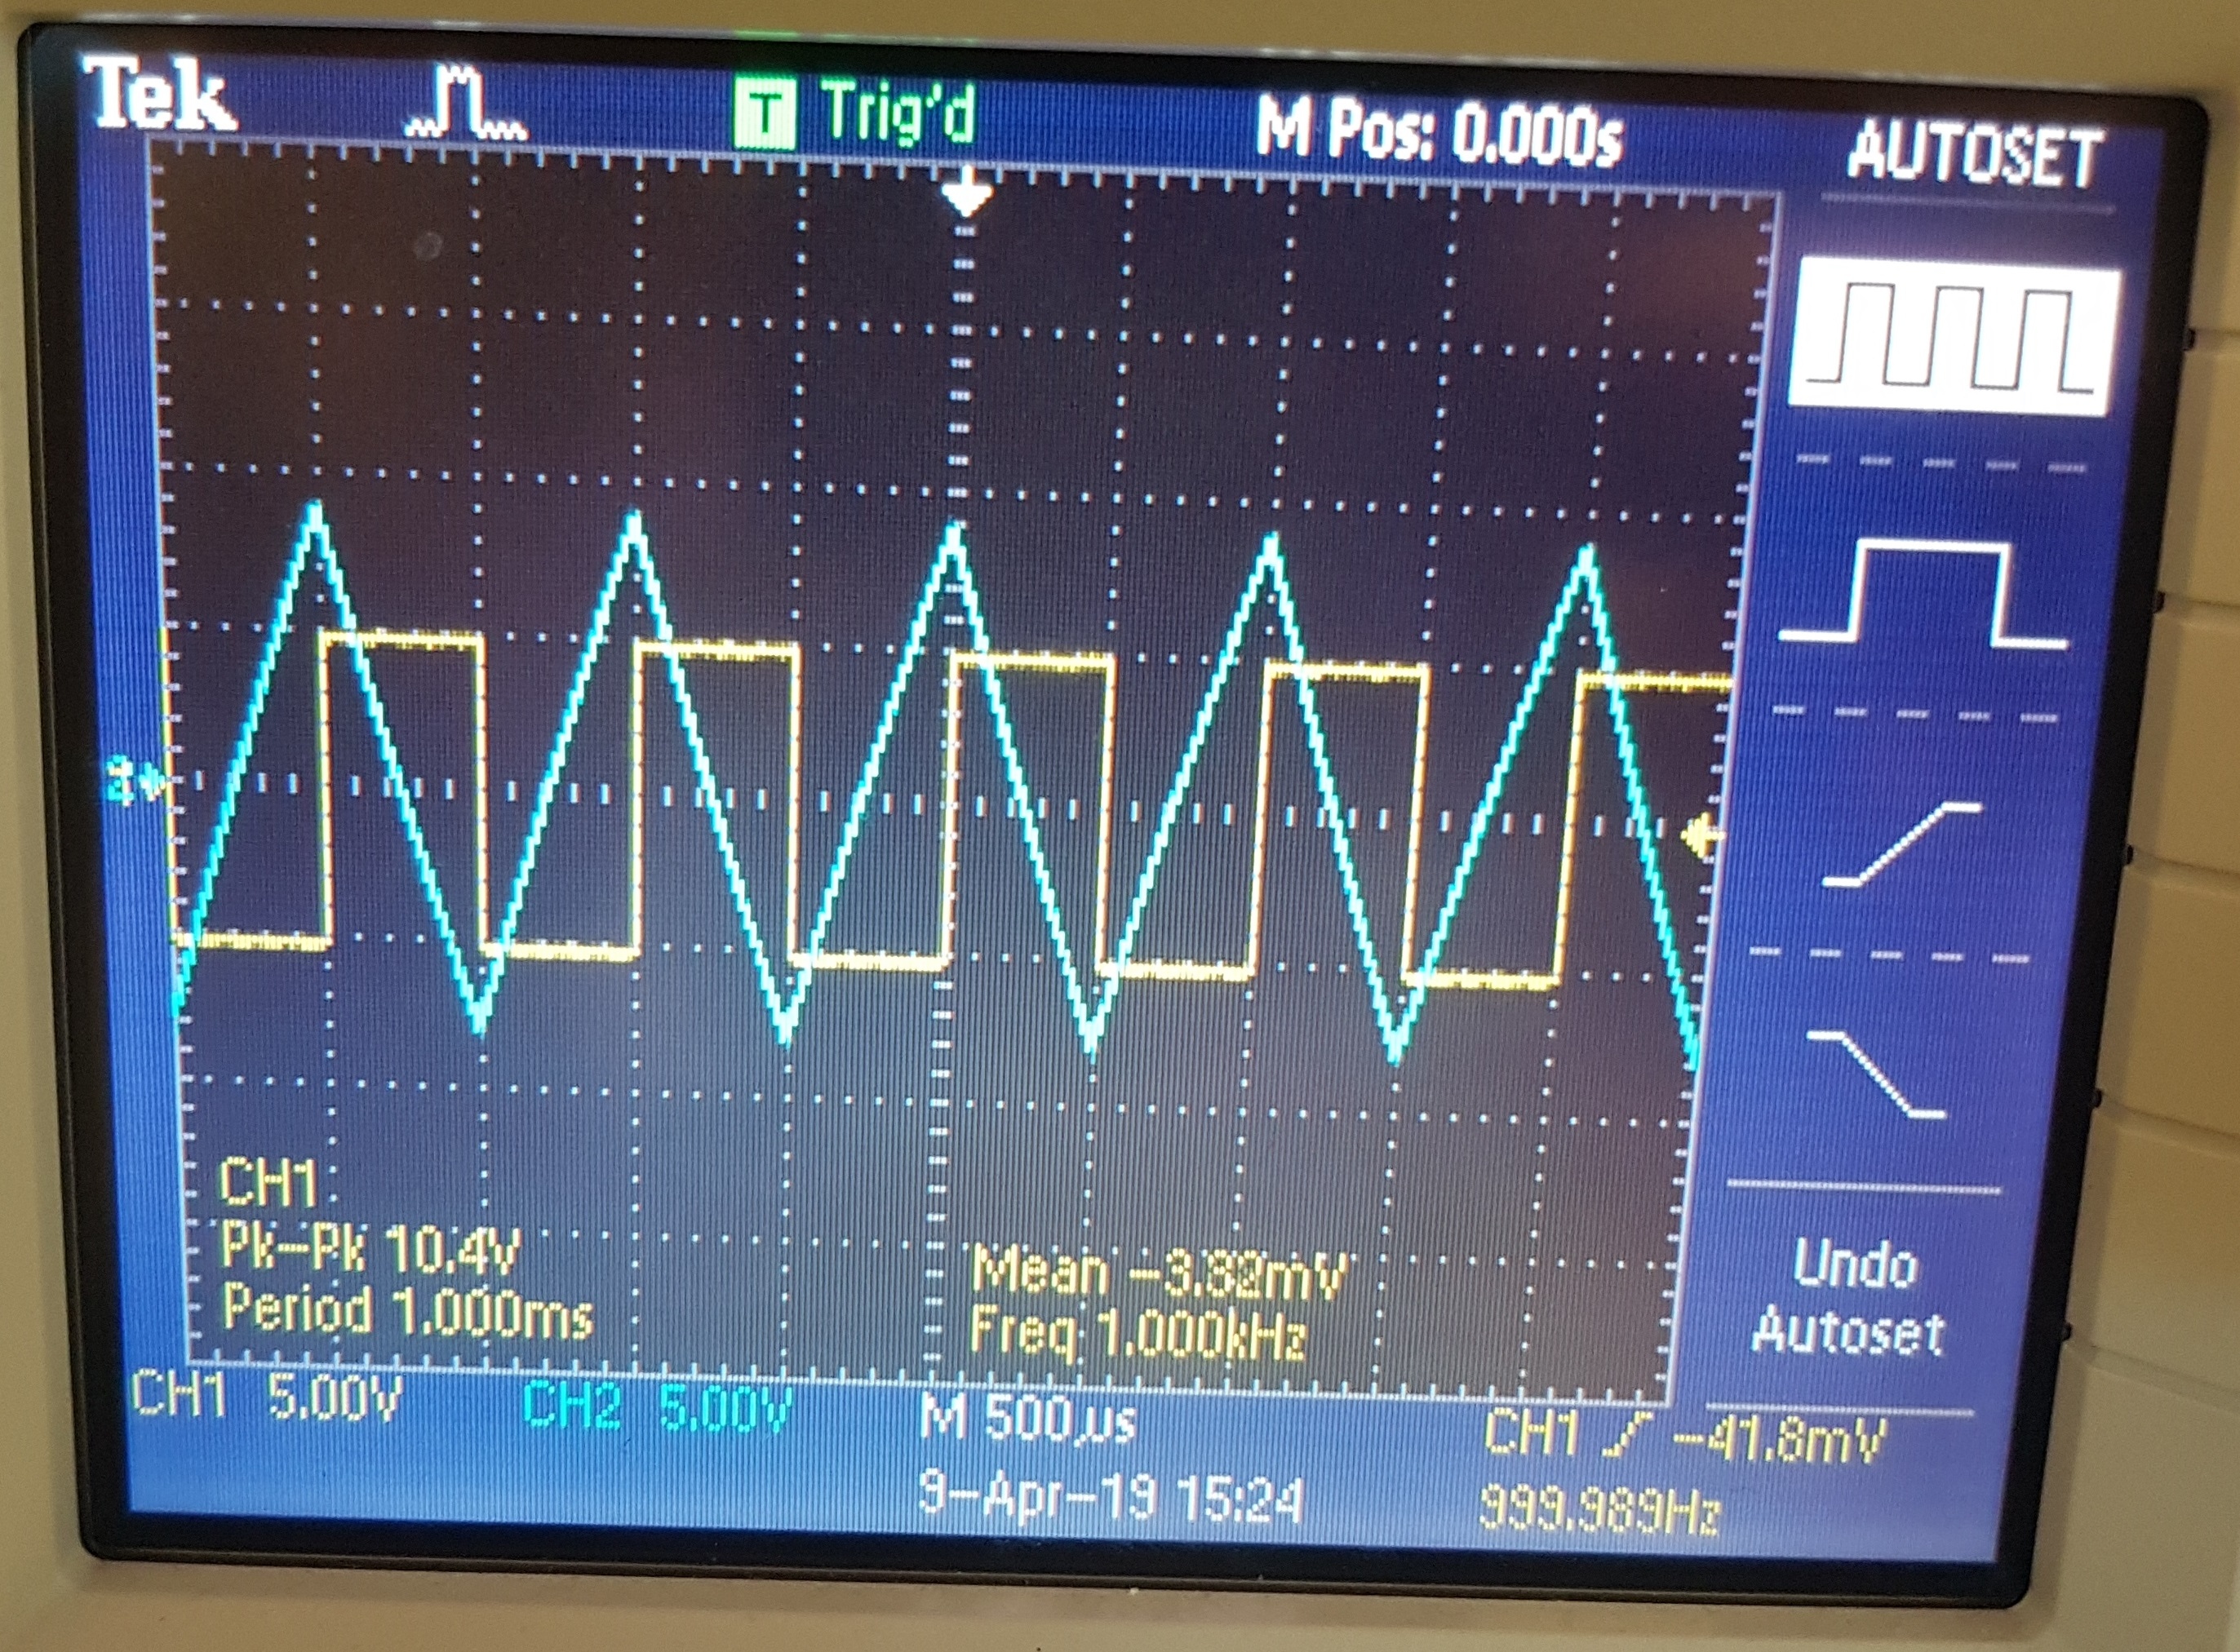
\includegraphics[width=0.6\linewidth]{Drifting}
				\caption{Output of integrator after a $10k\Omega$ was placed in parallel with the 							capacitor}
			\end{figure}
			The differences between figures 8, and figures 9 clearly show the impact of a dissipating 					resistor on reducing bias and wind-up.
		\item
			\textbf{Amplification}\\
			In figure 9 above, we used cursors to measure the gain of the integrator circuit, finding it 			to be close to 6dB, or a ratio of 1:2 from input to output. From this we know that the gain 				of the aplification OP-Amp must be -6dB or $\frac{1}{2}$ the original voltage.\\
			$\frac{V_{o}}{V_{i}} = \dfrac{-R_{2}}{R_{1}} \quad \therefore\quad \frac{V_{o}}{V_{i}} = 					\frac{1}{2} = \dfrac{-R_{2}}{R_{1}} \quad \therefore \quad -R_{2} = 2R_{1} $\\
			From this we know that if we chose $R_{2} = 20\Omega$ then $R_{1} = 10\Omega$
			producing the output seen in figure 10.
			
			\begin{figure}[ht]
				\centering
				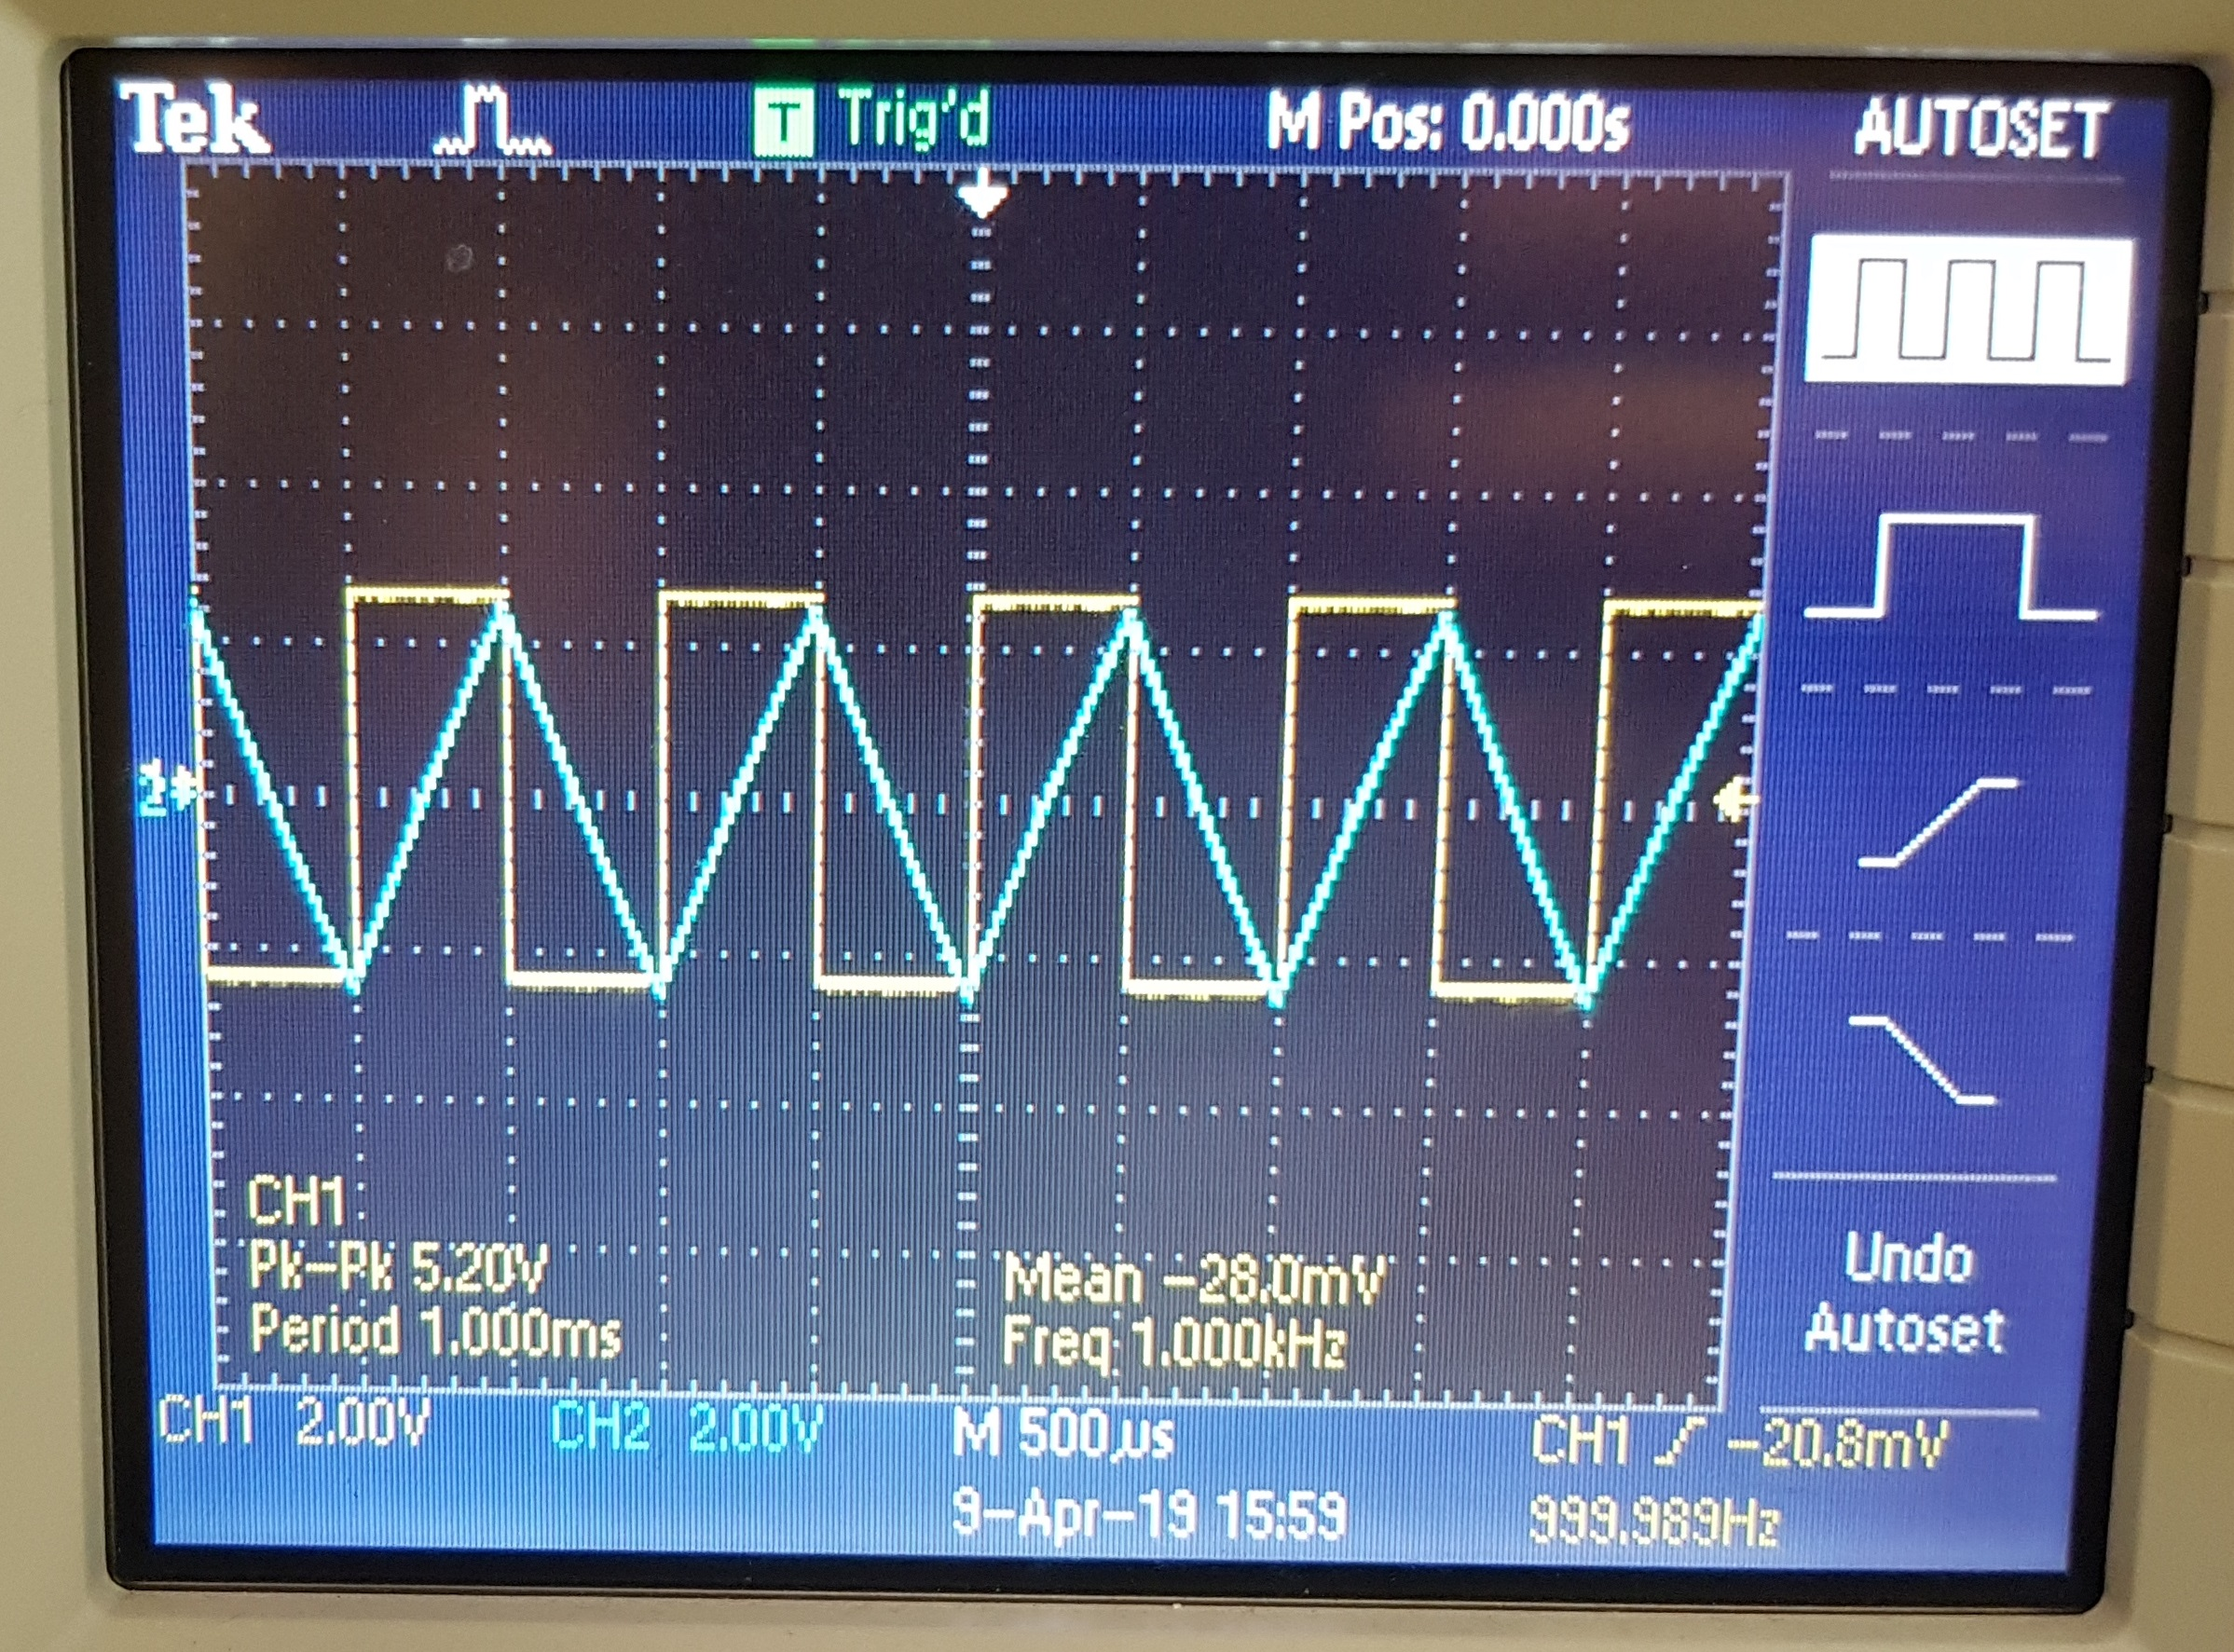
\includegraphics[width=0.6\linewidth]{Amplification_osc}
				\caption{Integrator output amplified by OP-Amp}
			\end{figure}
		\newpage
			\begin{figure}[ht]
				\centering
				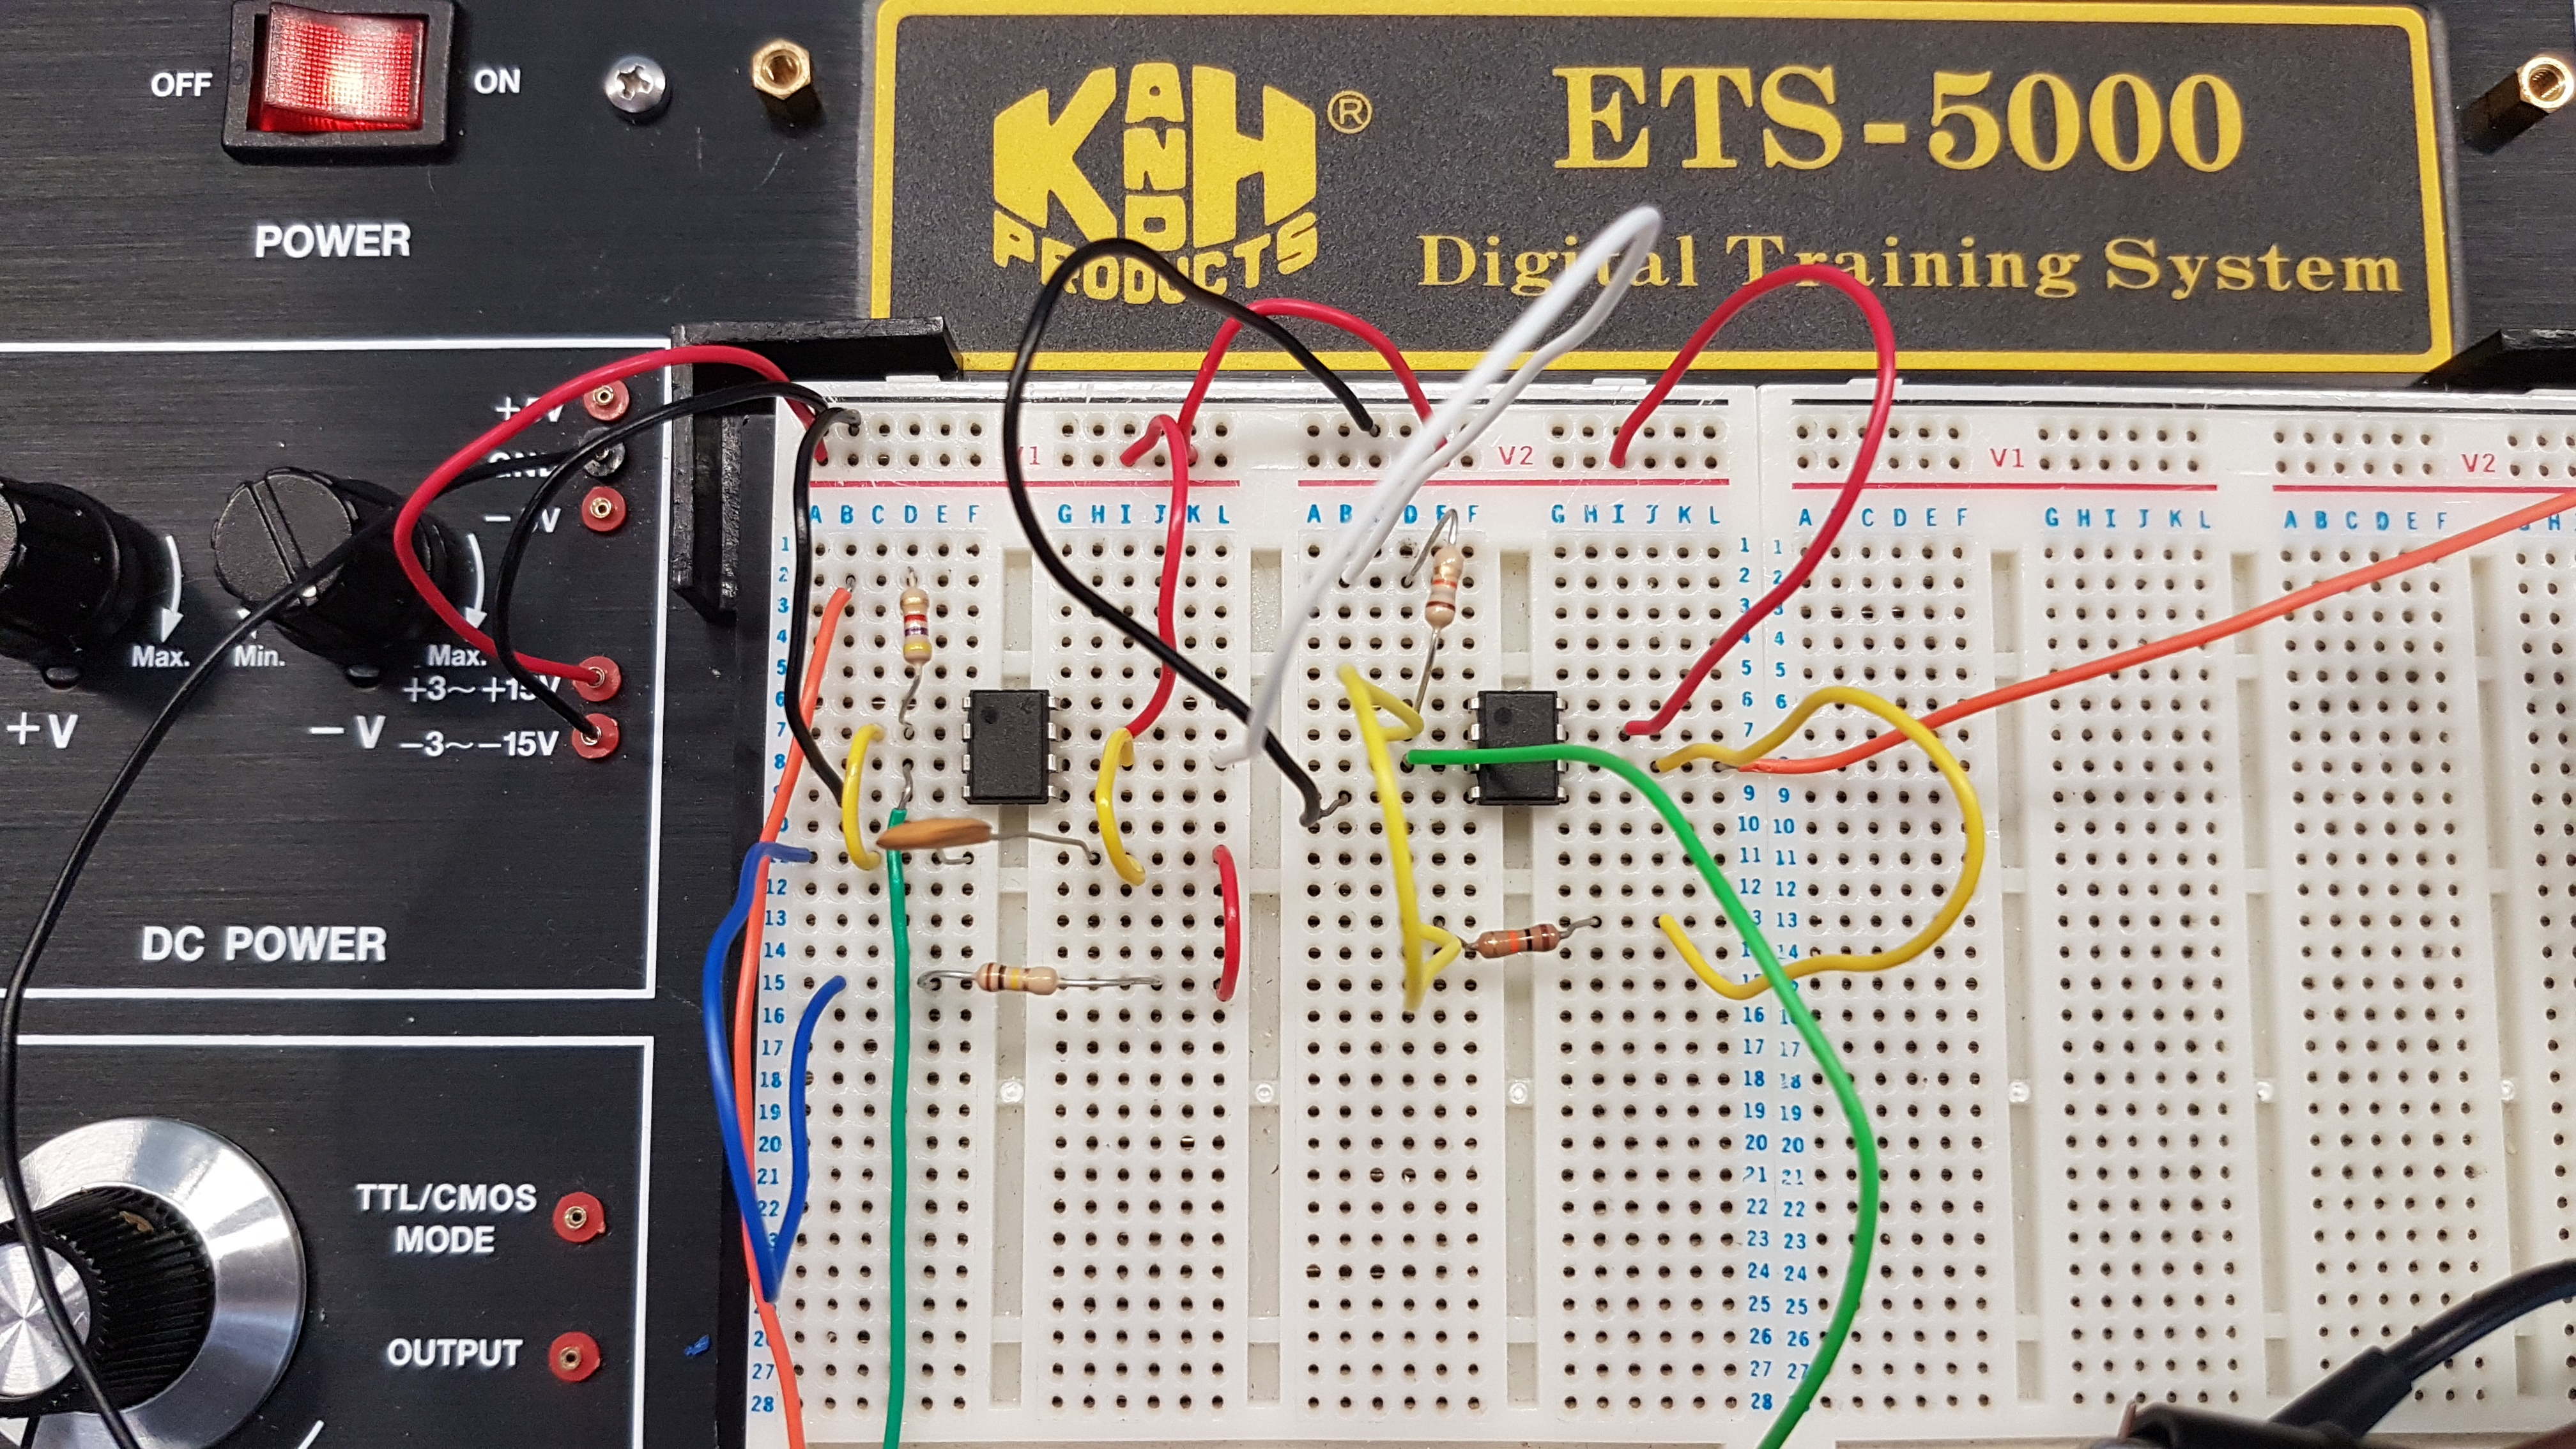
\includegraphics[width=\linewidth]{Apmlification}
				\caption{Integrator output amplified by OP-Amp, circuit on breadboard}
			\end{figure}
			
			
		\end{enumerate}			
			
	\end{flushleft}
\end{document}
